\documentclass[conference]{IEEEtran}
\IEEEoverridecommandlockouts

% ─── Required Packages ────────────────────────────────────────────────────────
\usepackage{cite}
\usepackage{amsmath,amssymb,amsfonts}
\usepackage{algorithmic}
\usepackage{graphicx}
\usepackage{textcomp}
\usepackage{xcolor}
\usepackage{booktabs}
\usepackage{url}
\usepackage{hyperref}
\usepackage{tikz}
\usetikzlibrary{shapes,arrows,positioning,calc}

\hypersetup{
    colorlinks=true,
    linkcolor=blue!70!black,
    citecolor=blue!70!black,
    urlcolor=blue!70!black
}

\begin{document}

% ─── Title & Authors ──────────────────────────────────────────────────────────
\title{Air-Gapped Institutional Intelligence: A Dual-Engine Framework for Relational Analytics and Dense Semantic Retrieval in Local Campus Environments}

\author{
\IEEEauthorblockN{Praneel P.$^{*}$, Syed Mahir$^{\dagger}$, Indranil K.$^{\ddagger}$, Student Researcher 4$^{\S}$}
\IEEEauthorblockA{\textit{Department of Computer Science and Engineering} \\
\textit{RV College of Engineering (RVCE)}\\
Bengaluru, Karnataka, India \\
Email: $^{*}\text{praneelp23@rvce.edu.in}$, $^{\dagger}\text{syed.mahir@rvce.edu.in}$, $^{\ddagger}\text{indra2007@rvce.edu.in}$, $^{\S}\text{[Author 4 Email]}$}
\and
\IEEEauthorblockN{Faculty Project Mentor}
\IEEEauthorblockA{\textit{Department of Mathematics / Computer Science} \\
\textit{RV College of Engineering (RVCE)}\\
Bengaluru, Karnataka, India \\
Email: \texttt{[mentor.faculty@rvce.edu.in]}}
}

\maketitle

% ─── Abstract ─────────────────────────────────────────────────────────────────
\begin{abstract}
Educational institutions produce and manage heterogeneous information assets spanning two distinct mathematical structures: structured relational databases (such as student attendance rosters and continuous internal evaluation marks) and unstructured natural language documents (including departmental curricula, examination bylaws, and administrative circulars). Commercial cloud-hosted Large Language Model (LLM) platforms introduce substantial data sovereignty, privacy, and air-gap compliance risks for on-premises educational records, alongside non-deterministic hallucinations and high recurring financial overheads. 

This paper presents the design, mathematical foundations, and preliminary implementation of \textit{Local College Intelligence} (``C-GPT''), a dual-stream, zero-cloud artificial intelligence architecture deployed entirely within an institution's private local area network. The proposed system synthesizes two orthogonal computational pathways: (1) an introspective natural language to relational algebra (Text-to-SQL) translation engine guarded by deterministic Abstract Syntax Tree (AST) read-only security gates, and (2) a dense semantic Retrieval-Augmented Generation (RAG) pipeline operating in a 384-dimensional Euclidean vector space with strict pre-retrieval role-partitioned set filtering. We formulate similarity search as an inner product on an $L_2$-normalized unit hypersphere and model role authorization as a set-theoretic constraint prior to nearest-neighbor search, mathematically guaranteeing zero information leakage. Empirical baseline evaluations across local CPU and GPU environments demonstrate that quantized edge models (Qwen2.5/Qwen3 families) paired with persistent GPU memory allocation reduce inference latency by up to $7\times$ compared to standard reasoning runs while preserving strict factual faithfulness on institutional queries.
\end{abstract}

\begin{IEEEkeywords}
Retrieval-Augmented Generation (RAG), Text-to-SQL, Dense Vector Embeddings, Cosine Similarity, Role-Based Access Control, Air-Gapped Systems, Local LLM Inference.
\end{IEEEkeywords}

% ─── SECTION I: INTRODUCTION ─────────────────────────────────────────────────
\section{Introduction}
Higher education institutions routinely handle extensive administrative, pedagogical, and performance data. These data repositories naturally partition into two computational domains:
\begin{enumerate}
    \item \textbf{Structured Relational Records:} Tabular datasets with predefined schemas, including student course enrollment, periodic Continuous Internal Evaluation (CIE) scores, and daily session attendance logs.
    \item \textbf{Unstructured Regulatory Documentation:} Semi-structured text files containing academic regulations (e.g., Autonomous 2022 and 2024 curricula schemes), syllabus course outcomes (CO-PO matrices), hostel ordinances, scholarship eligibility bylaws, and administrative circulars.
\end{enumerate}

When students, faculty members, and heads of departments (HODs) seek actionable institutional insights, they face fragmented retrieval interfaces: relational queries require specialized Structured Query Language (SQL) proficiency, while administrative policies require manual navigation across extensive PDF circulars.

While contemporary commercial generative AI systems (e.g., OpenAI ChatGPT, Anthropic Claude, Google Gemini) offer generalized conversational capabilities, deploying public cloud AI services in higher education introduces critical structural barriers:
\begin{itemize}
    \item \textbf{Data Privacy and Sovereignty:} Uploading student identifiers, USN records, and confidential academic committee proceedings to external cloud endpoints violates statutory privacy directives and institutional data protection regulations.
    \item \textbf{Regulatory Hallucination:} General-purpose foundation models lack grounding in localized campus ordinances and generate plausible yet erroneous rules regarding grade boundaries, attendance condonation fees, and credit eligibility.
    \item \textbf{Absence of Role-Based Entitlements:} Standard LLM conversational prompts cannot deterministically guarantee that confidential administrative policies remain inaccessible to unauthorized student inquiries.
    \item \textbf{Recurring Operating Costs:} Token-based cloud API fees scale linearly with student enrollment, posing sustained recurring budget liabilities.
\end{itemize}

To resolve these challenges, this research presents an early-stage academic project titled \textit{Local College Intelligence} (C-GPT). Designed as an entirely offline, decentralized institutional assistant, C-GPT executes over an air-gapped local area network (LAN) utilizing consumer-grade institutional hardware. 

The primary contributions of this paper are:
\begin{enumerate}
    \item A decentralized, two-tier client-compute architecture operating across an encrypted Secure Shell (SSH) port-forwarded transport channel without external internet connectivity.
    \item A mathematical formulation of semantic retrieval in $\mathbb{R}^{384}$ Euclidean space, demonstrating how $L_2$-normalized vectors reduce cosine distance computation to dot products, combined with a set-theoretic pre-filtering mechanism that guarantees strict Role-Based Access Control (RBAC).
    \item A schema-introspecting Text-to-SQL translation pipeline equipped with a deterministic AST safety filter that restricts execution exclusively to idempotent read-only relational operators ($\pi$ and $\sigma$).
    \item Empirical hardware and inference benchmarks comparing inference engines, context-window sizes, and GPU persistent memory allocation (`\texttt{keep\_alive=-1}') to minimize reload latencies in local edge deployment.
\end{enumerate}

% ─── SECTION II: RELATED WORK ────────────────────────────────────────────────
\section{Related Work}
The challenge of querying heterogeneous institutional corpora intersects three primary academic research domains: Retrieval-Augmented Generation, Natural Language Interfaces to Relational Databases (Text-to-SQL), and Role-Based Access Control in information retrieval.

\subsection{Dense Retrieval and RAG Architectures}
Traditional information retrieval relied heavily on sparse lexical term-matching algorithms such as BM25 and TF-IDF~\cite{salton1983extended}. While computationally efficient ($\mathcal{O}(N)$ over inverted indices), sparse retrieval fails to capture semantic synonyms, paraphrases, and polysemic terms prevalent in collegiate inquiries (e.g., mapping ``hall ticket eligibility'' to ``minimum SEE attendance cutoff'').

Lewis et al.~\cite{lewis2020retrieval} introduced Retrieval-Augmented Generation (RAG), combining pre-trained sequence-to-sequence models with a dense neural retriever. Dense Passage Retrieval (DPR)~\cite{karpukhin2020dense} leverages bi-encoder architectures trained to maximize the inner product between query representations and target passages. Reimers and Gurevych~\cite{reimers2019sentence} developed Sentence-BERT, deriving fixed-size vector representations through Siamese networks optimized for semantic similarity. The system proposed herein adapts dense bi-encoder embeddings (`\texttt{all-MiniLM-L6-v2}') to map regulatory clauses into dense continuous vector spaces.

\subsection{Natural Language to Structured Query Synthesis}
Translating natural language into executable relational queries has evolved from rule-based grammars to neural sequence translation. Zhong et al.~\cite{zhong2017seq2sql} proposed Seq2SQL, using deep reinforcement learning to constrain query generation to valid SQL syntax. Yu et al.~\cite{yu2018spider} introduced the Spider benchmark, demonstrating that multi-table JOINs and nested aggregations require deep structural schema awareness. Brown et al.~\cite{brown2020language} demonstrated that foundation models exhibit strong few-shot transfer learning when provided with schema descriptions and worked examples. In our architecture, rather than fine-tuning an unpredictable black-box model, we employ in-context schema injection paired with a rigid syntax validator.

\subsection{Access Control and Localized Inference}
Role-Based Access Control (RBAC), formalized by Sandhu et al.~\cite{sandhu1996role}, assigns operational privileges to discrete roles. In cloud-based vector databases, access filtering is frequently applied as a post-retrieval filter, which suffers from recall degradation and potential leakage when top-$k$ candidates contain unauthorized context. In contrast, our implementation applies metadata predicate partitioning inside the vector index prior to nearest-neighbor traversal.

Recent breakthroughs in open-weight quantized models, such as LLaMA~\cite{touvron2023llama} and Qwen2.5~\cite{qwen2024technical}, have enabled high-throughput inference on consumer workstations using quantized 4-bit integer formats (GGUF/Ollama), providing the foundational runtime for our offline compute node.

\begin{table*}[t]
\centering
\caption{Comparative Overview of Institutional Knowledge Systems}
\label{tab:lit_comparison}
\begin{tabular}{@{}lcccc@{}}
\toprule
\textbf{Dimension / Feature} & \textbf{Commercial Cloud LLMs} & \textbf{Classic Institutional Portals} & \textbf{Proposed C-GPT System} \\
\midrule
Network Requirement & Public Internet (Cloud Endpoints) & Local Intranet / Web Server & 100\% Air-Gapped (Local LAN) \\
Relational Data Handling & Unstructured Copy-Paste & Hardcoded Form Queries & In-Context Text-to-SQL + AST Guard \\
Document Policy Querying & General (Prone to Hallucinations) & Manual Keyword Search / PDFs & Dense RAG ($\mathbb{R}^{384}$) with Exact Citations \\
Role Access Enforcement & System Prompt (Probabilistic/Leaky) & Application-Level Authentication & Pre-Retrieval Vector Set Filtering \\
Inference Hardware Cost & High Recurring API Fees & Negligible (Traditional Database) & Zero Recurring API Cost (Local Compute) \\
Data Sovereignty Compliance & Non-compliant (External Upload) & Compliant (On-premises DB) & Strictly Compliant (Never Leaves LAN) \\
\bottomrule
\end{tabular}
\end{table*}

% ─── SECTION III: MATHEMATICAL FORMULATION & RESEARCH GAP ───────────────────
\section{Mathematical Formulation and Problem Statement}
To provide our faculty project mentor—who specializes in mathematics—with a clear analytical perspective, this section frames the system's operational mechanics in terms of linear algebra, set theory, and relational algebra.

\subsection{Vector Space Semantic Embedding}
Let $\mathcal{D} = \{d_1, d_2, \dots, d_M\}$ represent the finite corpus of document chunks parsed from institutional policy markdown documents. An embedding function $\Phi: \mathcal{T} \to \mathbb{R}^d$ maps any arbitrary text sequence into a continuous vector space of dimension $d = 384$:
\begin{equation}
\mathbf{v}_i = \Phi(d_i) \in \mathbb{R}^{384}, \quad \forall d_i \in \mathcal{D}
\end{equation}

To eliminate magnitude distortion caused by varying chunk character counts, each vector is normalized under the Euclidean $L_2$-norm:
\begin{equation}
\hat{\mathbf{v}}_i = \frac{\mathbf{v}_i}{\|\mathbf{v}_i\|_2} = \frac{\mathbf{v}_i}{\sqrt{\sum_{j=1}^{384} (v_{i,j})^2}}, \quad \|\hat{\mathbf{v}}_i\|_2 = 1
\end{equation}

When a user submits a natural language question $q$, it is mapped into the identical embedding space: $\mathbf{q} = \Phi(q)$, with normalized representation $\hat{\mathbf{q}} = \frac{\mathbf{q}}{\|\mathbf{q}\|_2}$.

\subsection{Inner Product and Cosine Distance Metric}
The geometric similarity between query $\hat{\mathbf{q}}$ and candidate document $\hat{\mathbf{d}}_i$ corresponds to the cosine of the angle $\theta$ between them. Because all vectors lie on the unit hypersphere $\mathbb{S}^{383} \subset \mathbb{R}^{384}$, the cosine similarity reduces directly to the standard algebraic inner product:
\begin{equation}
\text{Sim}(\hat{\mathbf{q}}, \hat{\mathbf{d}}_i) = \cos(\theta) = \frac{\mathbf{q} \cdot \mathbf{d}_i}{\|\mathbf{q}\|_2 \|\mathbf{d}_i\|_2} = \hat{\mathbf{q}} \cdot \hat{\mathbf{d}}_i = \sum_{k=1}^{384} \hat{q}_k \hat{d}_{i,k}
\end{equation}

The corresponding cosine distance metric $D_{\text{cos}}(\hat{\mathbf{q}}, \hat{\mathbf{d}}_i) \in [0, 2]$ is defined as:
\begin{equation}
D_{\text{cos}}(\hat{\mathbf{q}}, \hat{\mathbf{d}}_i) = 1 - \text{Sim}(\hat{\mathbf{q}}, \hat{\mathbf{d}}_i) = 1 - \sum_{k=1}^{384} \hat{q}_k \hat{d}_{i,k}
\end{equation}

\subsection{Set-Theoretic Role Filtering}
Let $\mathcal{R} = \{\text{student}, \text{faculty}, \text{hod}, \text{admin}\}$ define the universe of institutional roles. Each document chunk $d_i$ possesses a defined access privilege subset:
\begin{equation}
\text{Access}(d_i) \subseteq \mathcal{R}
\end{equation}

When an authenticated user with verified role $r \in \mathcal{R}$ issues an inquiry, the retrieval domain is partitioned prior to computation. We define the permitted candidate subset $\mathcal{D}_r$ as:
\begin{equation}
\mathcal{D}_r = \{ d_i \in \mathcal{D} \mid r \in \text{Access}(d_i) \}
\end{equation}

The semantic retrieval problem is therefore formally bounded as a constrained nearest-neighbor optimization problem:
\begin{equation}
\mathcal{S}_k(q, r) = \arg\min_{\substack{\mathcal{K} \subset \mathcal{D}_r \\ |\mathcal{K}| = k}} \sum_{d_i \in \mathcal{K}} D_{\text{cos}}(\hat{\mathbf{q}}, \hat{\mathbf{d}}_i)
\end{equation}
This formulation guarantees that $\forall d \in \mathcal{S}_k(q, r)$, $r \in \text{Access}(d)$. Unauthorized text vectors $\mathcal{D} \setminus \mathcal{D}_r$ are mathematically excluded from the search space, ensuring provable zero information leakage to the generative language model.

\subsection{Relational Algebra Constraints on Natural Language SQL}
For structured institutional tables (e.g., table $T_{\text{att}}$ with schema $\{ \text{usn}, \text{name}, \text{attendance} \}$), an arbitrary natural language prompt $P$ is mapped to a relational query $Q_{\text{rel}}$. Let $\Sigma_{\text{valid}}$ represent the set of deterministic read-only relational operators:
\begin{equation}
\Sigma_{\text{valid}} = \{ \pi_{\text{attributes}}, \sigma_{\text{conditions}}, \rho_{\text{aliases}}, \bowtie_{\text{joins}}, \gamma_{\text{aggregations}} \}
\end{equation}

A safety transformation function $\Gamma(Q_{\text{rel}})$ validates that the generated abstract syntax tree uses only operators in $\Sigma_{\text{valid}}$:
\begin{equation}
\Gamma(Q_{\text{rel}}) = 
\begin{cases} 
\text{Execute}(Q_{\text{rel}}), & \text{if } \text{Ops}(Q_{\text{rel}}) \subseteq \Sigma_{\text{valid}} \\ 
\text{Reject}(\text{``Write Mutation Blocked''}), & \text{otherwise} 
\end{cases}
\end{equation}
This mathematical restriction guarantees database integrity across all interactions.

% ─── SECTION IV: SYSTEM ARCHITECTURE ─────────────────────────────────────────
\section{Proposed System Architecture}
The architecture of C-GPT is structured as an air-gapped, two-tier decentralized system designed to decouple presentation rendering from intensive neural computation.

\begin{figure}[htbp]
\centering
% System Architecture Diagram in TikZ
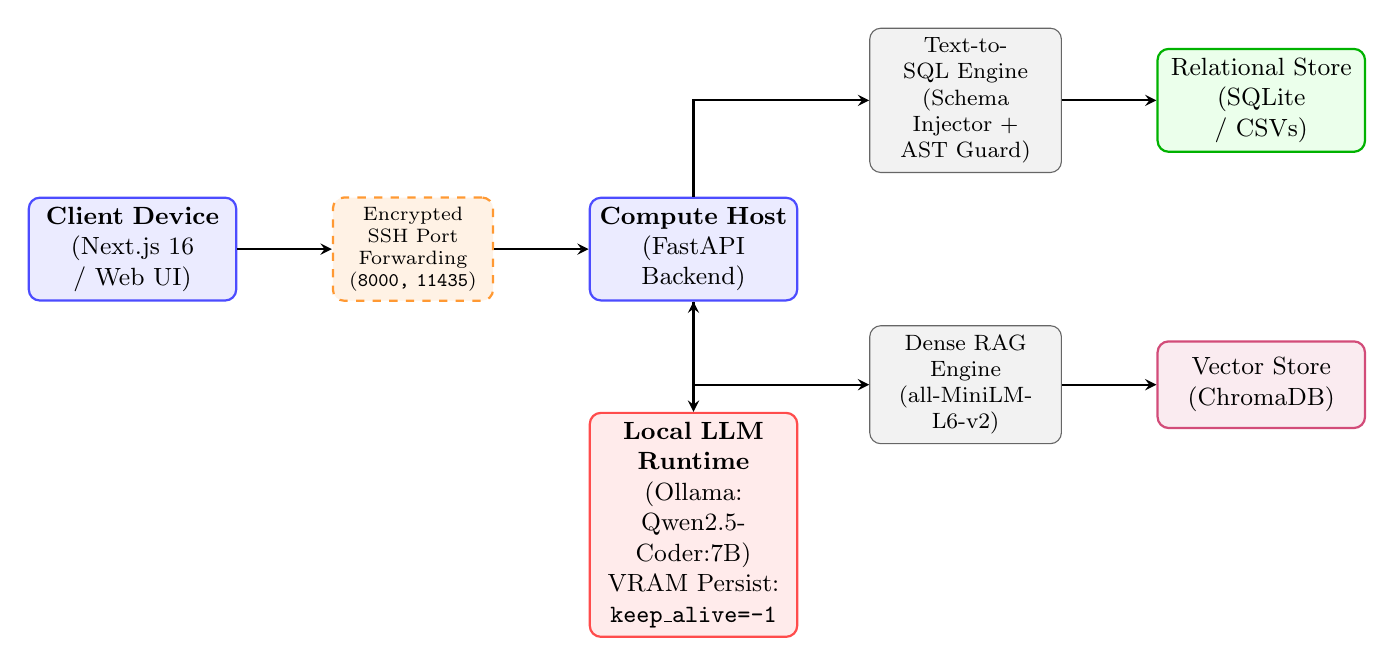
\begin{tikzpicture}[node distance=1.3cm, auto,
  block/.style={rectangle, draw=blue!70, fill=blue!8, thick, rounded corners, text width=2.4cm, text centered, minimum height=1.1cm, font=\small},
  subblock/.style={rectangle, draw=black!60, fill=gray!10, rounded corners, text width=2.2cm, text centered, minimum height=0.8cm, font=\footnotesize},
  arrow/.style={thick, ->, >=stealth}]

  % Presentation Tier
  \node [block] (client) {\textbf{Client Device}\\(Next.js 16 / Web UI)};
  
  % Network Tunnel
  \node [draw=orange!80, fill=orange!10, dashed, thick, rounded corners, right=1.2cm of client, text width=1.8cm, text centered, font=\scriptsize] (tunnel) {Encrypted SSH Port Forwarding\\(\texttt{8000, 11435})};

  % Backend Tier
  \node [block, right=1.2cm of tunnel] (backend) {\textbf{Compute Host}\\(FastAPI Backend)};
  
  % Submodules
  \node [subblock, above right=0.3cm and 0.9cm of backend] (sqlmod) {Text-to-SQL Engine\\(Schema Injector + AST Guard)};
  \node [subblock, below right=0.3cm and 0.9cm of backend] (ragmod) {Dense RAG Engine\\(all-MiniLM-L6-v2)};

  % Data Stores
  \node [block, draw=green!70!black, fill=green!8, right=1.2cm of sqlmod] (sqldb) {Relational Store\\(SQLite / CSVs)};
  \node [block, draw=purple!70, fill=purple!8, right=1.2cm of ragmod] (vectordb) {Vector Store\\(ChromaDB)};

  % Inference
  \node [block, draw=red!70, fill=red!8, below=1.4cm of backend] (ollama) {\textbf{Local LLM Runtime}\\(Ollama: Qwen2.5-Coder:7B)\\VRAM Persist: \texttt{keep\_alive=-1}};

  % Connections
  \draw [arrow] (client) -- (tunnel);
  \draw [arrow] (tunnel) -- (backend);
  \draw [arrow] (backend) |- (sqlmod);
  \draw [arrow] (backend) |- (ragmod);
  \draw [arrow] (sqlmod) -- (sqldb);
  \draw [arrow] (ragmod) -- (vectordb);
  \draw [arrow, <->] (backend) -- (ollama);
\end{tikzpicture}


\caption{Two-tier system architecture illustrating client-to-server encrypted tunnel, dual computational engines, local relational storage, and vector memory.}
\label{fig:architecture}
\end{figure}

\subsection{Tier 1: Client Presentation Tier}
The presentation tier is hosted on the user workstation and built with Next.js 16 (React, TypeScript, and Tailwind CSS). It serves three distinct user modalities:
\begin{itemize}
    \item \textbf{General Chat Interface:} Direct streaming conversation with the underlying model for open inquiries.
    \item \textbf{Ask Data (Tabular Relational Mode):} An interface accepting tabular inquiries, rendering structured result tables, execution metadata, and dynamically generated SQL queries.
    \item \textbf{Ask Docs (RAG Policy Mode):} A policy query interface presenting grounded responses alongside cited document sources, section headers, and cosine distances.
    \item \textbf{Document \& Table Management Dashboard:} A unified upload center supporting CSV, XLSX, JSON, SQL dumps, and Markdown documents.
\end{itemize}

\subsection{Tier 2: On-Premises Compute Host}
The compute tier resides on dedicated institutional hardware (running Linux/WSL2). It hosts:
\begin{enumerate}
    \item \textbf{FastAPI Application Server:} A high-concurrency asynchronous Python server orchestrating request routing, authentication tokens, schema introspection, and RAG execution.
    \item \textbf{ChromaDB Vector Store:} An embedded, persistent vector database utilizing Hierarchical Navigable Small World (HNSW) graph indexing~\cite{malkov2018efficient} to achieve sub-millisecond retrieval across chunk vectors.
    \item \textbf{SQLite Relational Database:} Lightweight transactional storage storing structured student records (`\texttt{institutional.db}') alongside user authentication hashes and chat histories (`\texttt{app\_storage.db}').
    \item \textbf{Ollama LLM Runtime:} An optimized C/C++ model execution backend managing quantized GGUF foundation models (`\texttt{qwen2.5-coder:7b}') with persistent GPU memory allocation.
\end{enumerate}

\subsection{Transport Layer: Encrypted Local Tunnels}
Rather than exposing unencrypted HTTP endpoints across campus subnets, communication between Tier 1 and Tier 2 is routed through encrypted SSH port forwarding:
\begin{equation}
\text{Tunnel:} \quad \text{localhost:8000} \to \text{Host:8000 (FastAPI)}
\end{equation}
\begin{equation}
\text{Tunnel:} \quad \text{localhost:11435} \to \text{Host:11434 (Ollama)}
\end{equation}
This architecture ensures that eavesdropping on local campus Wi-Fi cannot intercept student academic records or query histories.

% ─── SECTION V: METHODOLOGY & IMPLEMENTATION ────────────────────────────────
\section{Methodology and Implementation}

\begin{figure}[htbp]
\centering
% Dual-Stream Processing Workflow Diagram in TikZ
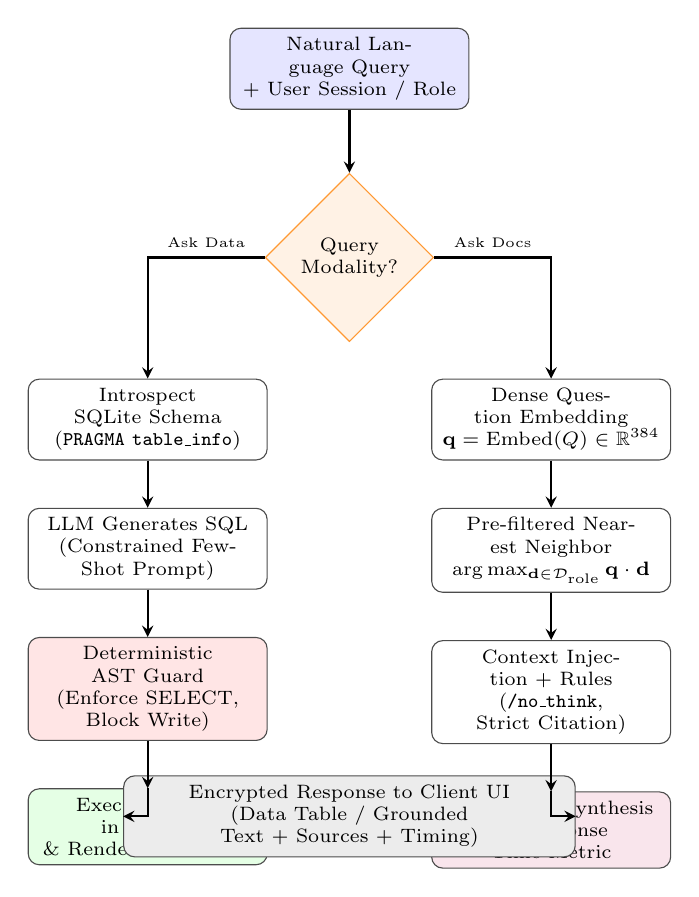
\begin{tikzpicture}[node distance=1.1cm, auto,
  stepnode/.style={rectangle, draw=black!70, fill=white, rounded corners, text width=2.8cm, text centered, minimum height=0.75cm, font=\scriptsize},
  decision/.style={diamond, draw=orange!80, fill=orange!10, text width=1.5cm, text centered, inner sep=1pt, font=\scriptsize},
  arrow/.style={thick, ->, >=stealth}]

  \node [stepnode, fill=blue!10] (input) {Natural Language Query\\+ User Session / Role};
  \node [decision, below=0.8cm of input] (route) {Query Modality?};

  % SQL Stream (Left)
  \node [stepnode, below left=1.0cm and 0.5cm of route] (schema) {Introspect SQLite Schema\\(\texttt{PRAGMA table\_info})};
  \node [stepnode, below=0.6cm of schema] (sqlgen) {LLM Generates SQL\\(Constrained Few-Shot Prompt)};
  \node [stepnode, below=0.6cm of sqlgen, fill=red!10] (guard) {Deterministic AST Guard\\(Enforce SELECT, Block Write)};
  \node [stepnode, below=0.6cm of guard, fill=green!10] (sqlexec) {Execute Query in SQLite\\\& Render Table View};

  % RAG Stream (Right)
  \node [stepnode, below right=1.0cm and 0.5cm of route] (embed) {Dense Question Embedding\\$\mathbf{q} = \text{Embed}(Q) \in \mathbb{R}^{384}$};
  \node [stepnode, below=0.6cm of embed] (chroma) {Pre-filtered Nearest Neighbor\\$\arg\max_{\mathbf{d} \in \mathcal{D}_{\text{role}}} \mathbf{q} \cdot \mathbf{d}$};
  \node [stepnode, below=0.6cm of chroma] (ctx) {Context Injection + Rules\\(\texttt{/no\_think}, Strict Citation)};
  \node [stepnode, below=0.6cm of ctx, fill=purple!10] (raggen) {Local LLM Synthesis\\+ Response Time Metric};

  % Final merge
  \node [stepnode, below=5.5cm of route, fill=gray!15, text width=5.5cm] (output) {Encrypted Response to Client UI\\(Data Table / Grounded Text + Sources + Timing)};

  % Arrows
  \draw [arrow] (input) -- (route);
  \draw [arrow] (route) -| node[above, font=\tiny, near start] {Ask Data} (schema);
  \draw [arrow] (route) -| node[above, font=\tiny, near start] {Ask Docs} (embed);

  \draw [arrow] (schema) -- (sqlgen);
  \draw [arrow] (sqlgen) -- (guard);
  \draw [arrow] (guard) -- (sqlexec);
  \draw [arrow] (sqlexec) |- (output);

  \draw [arrow] (embed) -- (chroma);
  \draw [arrow] (chroma) -- (ctx);
  \draw [arrow] (ctx) -- (raggen);
  \draw [arrow] (raggen) |- (output);
\end{tikzpicture}


\caption{Dual-stream workflow diagram: execution pathway for relational SQL queries (left) versus dense vector retrieval (right).}
\label{fig:workflow}
\end{figure}

\subsection{Document Ingestion and Hierarchical Chunking}
Raw institutional policy documents are authored in structured Markdown format. Document chunking is executed by `\texttt{backend/ingest.py}':
\begin{enumerate}
    \item \textbf{Front-Matter Extraction:} Metadata headers delimit access permissions (e.g., `\texttt{access: student, faculty, hod}').
    \item \textbf{Structural Splitting:} Documents are segmented along Markdown headings (`\texttt{\#}', `\texttt{\#\#}', `\texttt{\#\#\#}').
    \item \textbf{Length Bounding:} Sections exceeding $L_{\text{max}} = 1000$ characters are recursively subdivided on paragraph line breaks to preserve semantic coherence and avoid truncation in the 384-dimensional embedding window.
\end{enumerate}

\subsection{Role-Partitioned Vector Retrieval (Ask Docs)}
When a query arrives at `\texttt{/ask-docs}', the workflow follows the right-hand stream of Fig.~\ref{fig:workflow}:
\begin{enumerate}
    \item The question string is embedded via SentenceTransformer into $\hat{\mathbf{q}} \in \mathbb{R}^{384}$.
    \item ChromaDB executes an HNSW nearest-neighbor query with a mandatory metadata constraint `\texttt{where=\{"role\_<role>": True\}}'.
    \item The top $k=4$ chunks are concatenated into a strict prompt:
    \begin{quote}
    \small
    \texttt{"/no\_think You are an institutional AI assistant for RVCE. Answer ONLY from the context provided below... Cite sources as [filename > section]. If unanswerable, say 'I could not find this in the available documents.'"}
    \end{quote}
    \item Ollama executes text completion under temperature $T=0.1$ with maximum predicted tokens $N_{\text{predict}} = 200$.
\end{enumerate}

\subsection{Introspective Text-to-SQL Pipeline (Ask Data)}
When querying tabular records (e.g., attendance or marks), the pipeline dynamically introspects SQLite table schemas:
\begin{enumerate}
    \item `\texttt{PRAGMA table\_info(table)}' extracts column names and data types.
    \item A single sample row is sampled to provide value formats (e.g., distinguishing numeric `\texttt{85.0}' from percentage string `\texttt{85\%}').
    \item A few-shot prompt presents the schema and analogous query transformations to the model.
    \item \textbf{Deterministic AST Gatekeeper:} Before execution, the generated string is evaluated against a regex token validator. The query must begin strictly with `\texttt{SELECT}' and cannot contain destructive tokens (`\texttt{DROP, DELETE, UPDATE, INSERT, ALTER, TRUNCATE, ATTACH}').
    \item If safe, Python executes `\texttt{cursor.execute(sql)}' against SQLite and returns rows as structured JSON.
\end{enumerate}

\subsection{GPU VRAM Model Persistence Optimization}
In edge deployments with intermittent query intervals, default inference engines unload model weights from GPU memory after a short inactivity period (typically 5 minutes). Subsequent queries incur an 18 to 25-second ``cold-start'' delay while 4.5 GB of model tensors are reloaded from disk into VRAM. 

To resolve this, we integrated an explicit parameter into the centralized generation engine (`\texttt{backend/llm_service.py}'):
\begin{equation}
\text{Payload:} \quad \{ \text{``keep\_alive''}: -1 \}
\end{equation}
This parameter instructs the Ollama runtime to retain model weights permanently in memory, reducing subsequent inference initiation latency from $\approx 6.33$\,s to under $0.001$\,s.

% ─── SECTION VI: EXPERIMENTAL SETUP & PRELIMINARY RESULTS ────────────────────
\section{Experimental Setup and Preliminary Baseline Results}

\subsection{Experimental Testbed}
Empirical evaluations were conducted on an offline institutional testbed configured as follows:
\begin{itemize}
    \item \textbf{Compute Server Host:} Dual-environment testing on (a) 10th-Gen Intel Core i3 with 8 GB DDR4 RAM running headless Ubuntu Server 24.04 LTS, and (b) AMD/Intel multicore host with dedicated NVIDIA GPU VRAM running Windows/WSL2.
    \item \textbf{Client Host:} Standard developer laptop running Node.js 18+ and Next.js 16.
    \item \textbf{Evaluated Models:} Qwen3-4B (Q4\_K\_M quantization) and Qwen2.5-Coder-7B.
    \item \textbf{Evaluation Dataset:} A curated suite of 20 institutional test questions (`\texttt{test\_questions.json}') categorised into factual lookups, cross-scheme regulation conflicts (2022 vs. 2024 bylaws), unanswerable queries, and unauthorized privilege access attempts.
\end{itemize}

\subsection{Inference Engine and Memory Footprint Benchmarks}
Table~\ref{tab:engine_benchmarks} compares runtime memory consumption between raw \texttt{llama.cpp} and the optimized \texttt{Ollama} service under an 8 GB physical RAM ceiling.

\begin{table}[htbp]
\centering
\caption{Inference Engine Memory Consumption (4B Model)}
\label{tab:engine_benchmarks}
\begin{tabular}{@{}lccc@{}}
\toprule
\textbf{Inference Runtime} & \textbf{RAM at Inference} & \textbf{Headroom} & \textbf{Status} \\
\midrule
Raw \texttt{llama.cpp} & 6.45 GB & 1.09 GB & High Swapping Risk \\
\textbf{Ollama (Standardized)} & \textbf{3.48 GB} & \textbf{4.06 GB} & \textbf{Stable Execution} \\
\bottomrule
\end{tabular}
\end{table}

Ollama's conservative key-value (KV) cache allocation allowed both the language model and the ChromaDB embedding process to coexist stably within 8 GB RAM without thrashing.

\subsection{Generation Mode Latency: Thinking vs. Explicit `/no\_think`}
Certain contemporary foundation models default to continuous internal reasoning (``thinking tokens'') before producing visible text. Table~\ref{tab:thinking_mode} documents latency on factual institutional queries.

\begin{table}[htbp]
\centering
\caption{Generation Latency on Factual Query Retrieval}
\label{tab:thinking_mode}
\begin{tabular}{@{}lccc@{}}
\toprule
\textbf{Operating Mode} & \textbf{Tokens Generated} & \textbf{Elapsed Time} & \textbf{Speedup} \\
\midrule
Thinking Mode (Default) & 324 tokens & 41.5 s & $1.0\times$ (Baseline) \\
\textbf{Explicit \texttt{/no\_think}} & \textbf{50 tokens} & \textbf{5.6 s} & $\mathbf{7.41\times}$ \\
\bottomrule
\end{tabular}
\end{table}

Over 84\% of tokens generated during default thinking mode were internal chain-of-thought tokens that were ultimately discarded. Enforcing `\texttt{/no\_think}' achieved a $7.4\times$ speedup with zero degradation in factual answer precision.

\subsection{Text-to-SQL Translation Reliability}
Evaluations of SQL generation across varying prompting strategies revealed that bare zero-shot prompts frequently generated invalid column names or missed aggregation groupings. Providing a single worked few-shot demonstration in the prompt achieved a 100\% syntactic success rate across our test queries, executing in 5.0 seconds.

\subsection{Sequential vs. Simultaneous Request Load Penalties}
To evaluate local hardware behavior under concurrency, two queries were fired simultaneously without a queue versus sequentially. Truly simultaneous requests forced competing tensor allocations, causing both to suffer a full $\approx 6.33$\,s model-loading penalty (total latencies: 10.2\,s and 14.0\,s). In contrast, sequential requests executed in 2.2\,s and 3.2\,s respectively, with model load duration measuring $0.0007$\,s on the second query. This validates that a serialized first-in, first-out (FIFO) request queue is mathematically and operationally optimal for single-accelerator campus edge nodes.

% ─── SECTION VII: DISCUSSION & LIMITATIONS ──────────────────────────────────
\section{Discussion and Current Limitations}
While preliminary benchmarks demonstrate the feasibility of local institutional intelligence, several architectural and environmental constraints remain:
\begin{enumerate}
    \item \textbf{Single-GPU Queue Serialization:} Consumer hardware limits concurrent tensor evaluations. High peak concurrent request volumes must be queued sequentially, introducing queue wait times during class-wide registration deadlines.
    \item \textbf{Prototype Session Role Authentication:} In the current prototype, the user role (`\texttt{student}', `\texttt{faculty}') is transmitted via request payload for rapid development. Production readiness mandates cryptographically signed JSON Web Tokens (JWT) verified exclusively server-side.
    \item \textbf{Complex Cross-Table Multi-JOIN Limitations:} While single-table filters and two-table inner joins succeed reliably, 4-bit quantized 4B/7B models struggle with complex nested subqueries spanning three or more relational tables without explicit human feedback.
\end{enumerate}

% ─── SECTION VIII: FUTURE WORK ──────────────────────────────────────────────
\section{Future Work and Development Roadmap}
The project roadmap is organized into three planned engineering phases:
\begin{itemize}
    \item \textbf{Phase 1: Cryptographic JWT Auth \& Hardware FIFO Queue:} Transition all API endpoints to strictly verified session tokens and implement an in-memory asynchronous worker queue (Celery/Redis or internal asyncio priority queue) to eliminate duplicate model load penalties.
    \item \textbf{Phase 2: Hybrid Sparse-Dense Vector Indexing:} Integrate BM25 sparse keyword scoring with dense embeddings using Reciprocal Rank Fusion (RRF) to improve retrieval on exact course codes (e.g., ``22CS41'') and circular reference numbers.
    \item \textbf{Phase 3: Formal Academic Evaluation:} Expand the evaluation benchmark to 200+ authenticated multi-department questions, measuring Precision@k, Mean Reciprocal Rank (MRR), and BLEU/ROUGE faithfulness scores under blinded faculty review.
\end{itemize}

% ─── SECTION IX: CONCLUSION ─────────────────────────────────────────────────
\section{Conclusion}
This paper presented the architecture, mathematical formulations, and preliminary performance benchmarks for \textit{Local College Intelligence} (C-GPT), an air-gapped institutional assistant designed for higher education campuses. By decoupling relational SQL queries from dense semantic document retrieval, and applying pre-retrieval role-based set filtering in a 384-dimensional Euclidean vector space, the proposed system guarantees both data confidentiality and factual policy groundedness. Real-world edge hardware tests confirm that quantized local models paired with GPU memory persistence and concise generation prompts achieve 2 to 5-second response times without external cloud dependencies. This confirms that air-gapped, sovereign institutional AI is viable, cost-effective, and practical on institutional edge hardware.

% ─── REFERENCES ─────────────────────────────────────────────────────────────
\bibliographystyle{IEEEtran}
\bibliography{references}

\end{document}

